\section{Metodologia}\label{sec:metodologia}

\begin{frame}{Coleta dos Dados}
	\begin{itemize}
		\item Ferramenta ApacheBench;
		\item ``ab -n X -c Y'';
		\item X = Requisições Totais;
		\item Y = Requisições Simultâneas.
	\end{itemize}
\end{frame}

\begin{frame}{Ambiente de Testes}
	\begin{block}{Máquinas Virtuais}
		\begin{itemize}
			\item VirtualBox;
			\item Debian 7;
			\item 2GB de RAM;
			\item 30GB de HD;
			\item 1 Núcleo.
		\end{itemize}
	\end{block} \pause
	\begin{block}{Hospedeiro}
		\begin{itemize}
			\item Computador Portátil;
			\item Intel Core i5-3337U @ 1,8Ghz - 4 Núcleos;
			\item 8GB de RAM;
			\item 1TB de HD.
		\end{itemize}
	\end{block}
\end{frame}

\begin{frame}{Definição Dos Valores Utilizados nos Testes}
	\begin{block}{Valores}
		\begin{itemize}
			\item Requisições Totais variando de 1.000 à 15.000 com salto de 
			1.000;
			\item Carga de 10, 20, 40 e 80 porcento.
		\end{itemize}
	\end{block}
\end{frame}

\begin{frame}{Definição Dos Valores Utilizados nos Testes}
	\begin{figure}
		\centering
		\caption{Requisições Totais e Requisições Concorrentes}
		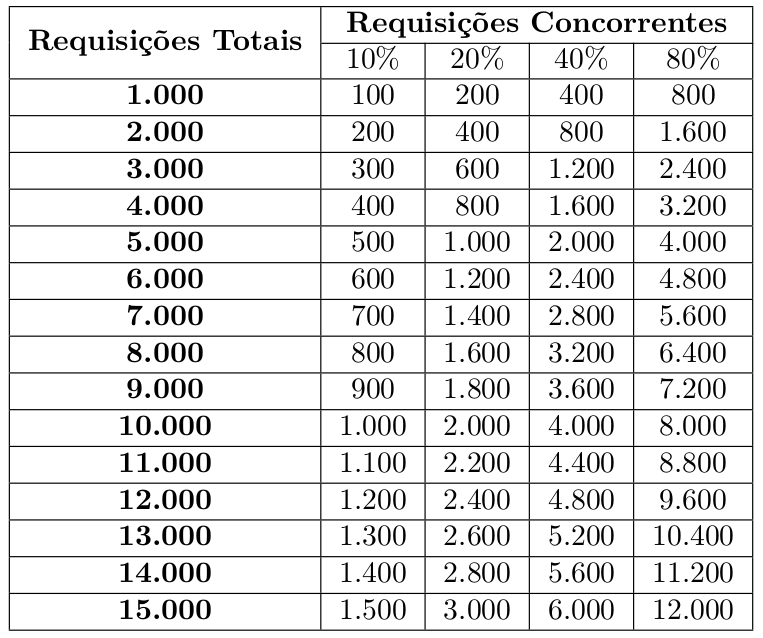
\includegraphics[width=0.7\linewidth]{tabela-requisicoes} \\
	\end{figure}
\end{frame}

\begin{frame}{Métricas Utilizadas}
As métricas utilizadas para comparar o desempenho dos servidores HTTP são as 
mesmas métricas calculadas e entregues pelo ApacheBench.
\begin{block}{Métricas}
\begin{itemize}
	\item Tempo total do teste em segundos (s);
	\item Total de dados transferido em bytes (b);
	\item Total de texto em HTML transferido em bytes (b);
	\item Tempo médio por requisição em milissegundos (ms);
	\item Tempo médio de resposta por requisição entre as requisições 
	concorrentes em milissegundos (ms);
	\item Taxa de transferência em Quilo Bytes por segundo (Kb/s).
\end{itemize}
\end{block}
\end{frame}





